\documentclass[10pt,a4paper]{article}
\usepackage[utf8]{inputenc}
\usepackage[german]{babel}
\usepackage[T1]{fontenc}
\usepackage{amsmath}
\usepackage{amsfonts}
\usepackage{amssymb}
\usepackage{graphicx}
\title{Gekoppelte Schwingungen}
\begin{document}
\section*{gekoppelte Schwingungen}
\begin{itemize}
\item Energieaustausch zwischen einzelnenen Oszillatoren ist möglich.
\item zum Beispiel zwei gekoppelte Pendel die durch Feder miteinander verbunden sind. $\Rightarrow$ neue Gleichgewichtslage.
\begin{figure}[hbtp]
\centering
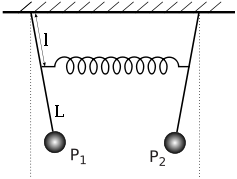
\includegraphics[scale=1]{coupled.png}
\end{figure}

\item $P_2$ wird um $\Theta_2$ ausgelenkt ausgelenkt. $ \Rightarrow M_2=-mgL\Theta_2-kl^2\Theta_2$ mit der Kopplungskonstante k.
\item $P_1$ wird um $\Theta_1$ ausgelenkt ausgelenkt. $ \Rightarrow M_2=-mgL\Theta_2-kl^2\Theta_2+kl^2\Theta_1=J\ddot{\Theta_2}$
\item dazu wurde verwendet, dass $M=J\ddot{\Theta}$ und für Pendel $J=mL^2$
\item Analoges Verfahren für $P_1$:
\begin{align*}
J\ddot{\Theta_1}=-mgL\Theta_1+kl^2(\Theta_2-\Theta_1) \\
J\ddot{\Theta_2}=-mgL\Theta_2+kl^2(\Theta_1-\Theta_2) \\
\Rightarrow \text{gekoppeltes Diffenzialgleichungssystem}
\end{align*}
\end{itemize}
\end{document}